\documentclass[12pt]{article}
\usepackage[a4paper, total={6in, 8in}]{geometry}
\usepackage{comment}
\usepackage{titling}
\usepackage{appendix}
\usepackage{pgfplots}
\usepackage{filecontents}

\title{Clustering for Graph Partitioning}
\author{Andrea Smith}

\begin{document}
\begin{titlingpage}
\setlength{\droptitle}{30pt}
\maketitle
\begin{center}
{\fontfamily{lmtt}\selectfont
\large\centerline{About the Author}
}
The author has earned her Bachelor's of Science degree in Computer Science from Missouri University of Science and Technology. She is working towards her doctorate degree in Computer Science, with a focus on graph data mining, from the same university, anticipating completing 2022.
\end{center}
\end{titlingpage}

\tableofcontents

\newpage
\section{Executive Summary}
This project aims to explore the potential of clustering algorithms for aiding in the partitioning of large graphs for frequent subgraph mining. Partitioning is important as many graphs of interest cannot be held in the memory of a single machine, and so must be spread across many machines in order to be processed. Partitioning risks losing data that spans across multiple partitions, requiring an intelligent partitioning process in order to minimize. 
\newline\newline
This project explores k-means clustering, distance-k clustering, and multilevel kernel clustering algorithms, as they apply to partitioning large transaction graphs in data mining. The clusters produced by the algorithms are evaluated for quality based on cluster density and the maximal shortest path within the cluster. The algorithms were tested on a toy data set built from publicly available Arabian horse pedigree papers, such that each edge represents a child-parent relationship. The algorithms were written for undirected, weighted graphs, but could be modified for directed graphs.
\newline\newline
Further research needs to be done to create and evaluate parallelized or distributed versions of these algorithms, so that they can process graphs that do not fit within the memory of a single machine.

\newpage
\section{Introduction}
Stuff to say \cite{kernel,distK}.

\newpage
\section{Project Specifications}
This project focuses on comparing the quality of the clusters produced by each algorithm. Quality is a combined score  of the cluster density and the maximum shortest path within the cluster. By comparing the clustering ability of the algorithms on a small graph, inferences about the quality of partitions made on a larger transaction graph can be made. Note that further research should be done into parallelized and distributed versions of these algorithms, but that is beyond the scope of this project.
\newline\newline
All code was written in the C++ programming language. The program accepts as input a properly formatted document file that describes the graph to execute. The program outputs the basic statistics of the clusters formed by each of the three algorithms, as well as a list of which nodes are in which cluster. The statistics reported include the number of clusters formed, the number of elements in each cluster, the density of each cluster, and the diameter of each cluster.
\newline\newline
In the future, the program should be modified to accept a parameter file that can affect the execution of the program. Parameters of interest would include the number of clusters that the k-means algorithm should search for, and the sigma value for the kernel clustering algorithm.

\newpage
\section{Detailed Design}
The program was designed in a combination of the object-oriented method and the functional method of programming.
\subsection{Class Objects}
The driving force of the program is a UndirectedGraph class, which is built from a SymmetricalMatrix class. The data is represented as an undirected graph because the project is looking for relationships between the horses, and we do not care about which horse is the parent. This then allows us to use a SymmetricalMatrix class, which is much more memory efficient to use than a full matrix class would be, as only either the upper or lower triangle of the matrix actually needs to be stored.
\newline\newline
While C++ has a basic vector class, it does not have any linear algebra functions attached to that class. Instead, a custom vector class was developed for use, which the basic Matrix class was then built on top of. This combination allows for full flexibility to implement any of the needed linear algebra operations directly into the class. This was designed to be used by a spectral clustering algorithm, but that algorithm has instead been removed from the scope of this project. The SymmetricalMatrix class inherits from the Matrix class, but was given more efficient memory management, to take advantage of the fact the half of the values in the matrix are identical. A simple UML diagram for the relationship between the custom classes exists in Appendix \ref{appendix:uml}.
\newline\newline
The UndirectedGraph class includes a SymmetricalMatrix object as a private member. This matrix is used to store the adjacency matrix of the undirected graph. The advantage to this method is realized in very dense graphs, as it becomes more efficient to store and to work with than other representations, which often involve long lists of node id pairs. Unfortunately, the graph used in the testing was not a particularly dense graph, and so this particular benefit did not come to light. However, dense graphs are a prioritized area of interest in the data mining field, and so it was important to consider that beyond this project.
\newline\newline
The C++ data type std::set was chosen to represent the clusters within the functional algorithms. The class type has a strict enforcement of no duplication within a set and supports simple insertion, deletion, and search operators. Each node was represented in the cluster by it's id in the original graph, not by it's string label, which is more efficient as string operations are cumbersome and slow.

\subsection{Algorithms}

\subsubsection{K-Means}
The k-means function was broken into five different sub-functions. This helps improve readability of the code and allowed some sections to be reused for the other algorithms. The pseudo-code for the k-means algorithm is represented in Appendix \ref{appendix:kmeans} and the pseudo-code for the k-means centroid initialization is presented in Appendix \ref{appendix:kmeansinit} \cite{kmeans}. For this application, the distance between two nodes is taken as the shortest path between them, and the center of the cluster is selected to be the node with the highest closeness centrality. For future comparison, it would be interesting to see if different clusters were created if the center of the cluster was calculated based on betweenness centrality.

\subsubsection{Distance-K}
The distance-k algorithm is different from the other two, in that instead of taking a parameter that describes the number of clusters to create, it takes a parameter that describes the maximum size a cluster can be. This particular algorithm was developed for non-euclidean graphs, and so the size of a cluster is known as the diameter of it. This is more often known as the longest shortest path between any two nodes in the cluster.
\newline\newline
The algorithm starts by forming clusters around the nodes that have the highest degree. It selects the highest degree node that is not already in a cluster, and forms a cluster of it and all of it's neighbors who are not already in clusters. Pseudo-code for this process can be found in Appendix \ref{appendix:distk_init}. Once this is done, the algorithm will attempt to merge clusters together until they are too big, according to the distance parameter. Once no more merges can be made, the algorithm completes \cite{kernel}.

\subsubsection{Kernel Clustering}
Kernel clustering is done in three steps. The first step is coarsening the data. This step lends itself well to recursion, as each level of coarseness does not need to know about any previous or next level. \newline\newline
The second step is initial clustering. Since any clustering method can be done here, k-means was selected for this project. While k-means is reliable, it does potentially change the data quality. It would have been more complete to run the Kernel Clustering algorithm twice, once with k-means and once with distance-k, or to have selected a third clustering algorithm entirely for kernel clustering.
\newline\newline
The third step of the algorithm is refinement. This requires a memory of the different levels of coarseness, in order to step back through them. Unfortunately, we did not think of a better way to solve this issue other than to hold in memory the different graphs created and a record of how the nodes were merged to reach that step. For large graphs, this could be a prohibitive amount of memory, especially with many iterations of coarsening.
\newline\newline
At each level of refinement of nodes, the clusters are also refined. The algorithm presented for this was a modified k-means algorithm \cite{kmeans}, which is expected to converge quickly at every iteration because the centroids received a good initialization due to the coarsening steps. The pseudo-code for the refinement of the clusters can be found in Appendix \ref{appendix:kernel_kmeans}.

\newpage
\section{Experimental Results}

\subsection{Experiment Setup}
The experiment run was a graph with 64 nodes of Arabian horse pedigree relationships, where an edge between two nodes indicated a parent-child relationship. Due to the fact that only one of the tested algorithms had a random element to it, multiple iterations were not recorded.

\subsection{Results Analysis}
The results of each algorithm can be seen in Figure \ref{results_data}. Our standards for quality involve balancing the average cluster density and size against average cluster diameter. Ideally, the algorithms should find large and dense clusters, with a short path to all nodes in the cluster.

\begin{figure}[!htb]
\begin{center}
	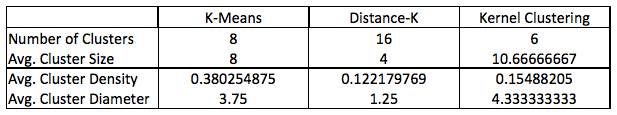
\includegraphics[height=7em]{data.png}
	\caption{Cluster Algorithm Results}
	\label{results_data}
\end{center}
\end{figure}

It can be seen in the results that while Kernel Clustering returned the largest clusters, they also had the largest diameter, and a relatively low density. So rather than tight clusters, it found very loose clusters. Conversely, K-Means easily had the best density within it's clusters, and was on the high end of the cluster size. Again, however, it tended on the high end of the cluster diameters.
\newline\newline
The Distance-k algorithm was notable in its very low average cluster diameter, but when examining the clusters themselves, the algorithm placed many nodes in clusters of one or two, thus very much lowering all three values collectively.

\subsection{Difficulties}
One of the main difficulties of this program was evaluating the calculated clusters for correctness. A visual aid tool was not developed, so all clusters had to be manually checked against the original matrix and drawn by hand during the development and testing process. For continued work, a visualization tool would need to be integrated or developed.

\newpage
\appendix
\appendixpage
\addappheadtotoc

\section{UML Diagram for Custom Classes}
\label{appendix:uml}
\begin{figure}[!htb]
\begin{center}
	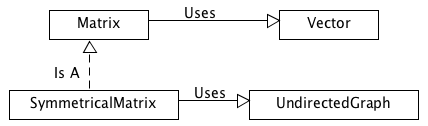
\includegraphics[height=10em]{uml.png}
	\caption{UML Diagram for Relationships between Class Types}
\end{center}
\end{figure}

\newpage
\section{Pseudo-Code for the K-Means Algorithm}
\label{appendix:kmeans}
\begin{figure}[!htb]
\begin{center}
	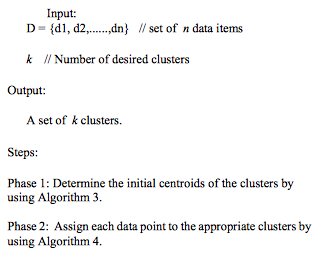
\includegraphics[height=25em]{kmeans.png}
	\caption{Pseudo-Code for the K-Means Algorithm}
\end{center}
\end{figure}

\newpage
\section{Pseudo-Code for the K-Means Cluster Initialization Algorithm}
\label{appendix:kmeansinit}
\begin{figure}[!htb]
\begin{center}
	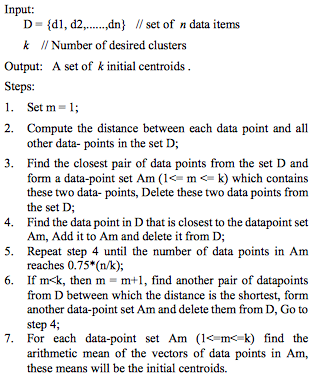
\includegraphics[height=30em]{kmeans_init.png}
	\caption{Pseudo-Code for the K-Means Cluster Initialization Algorithm}
\end{center}
\end{figure}

\newpage
\section{Pseudo-Code for the Kernel K-Means Refinement Algorithm}
\label{appendix:kernel_kmeans}
\begin{figure}[!htb]
\begin{center}
	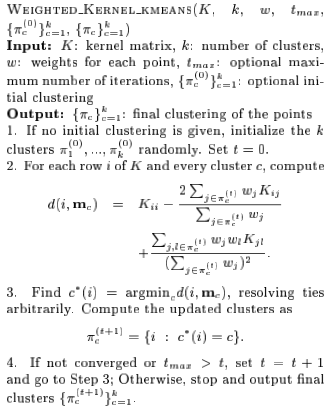
\includegraphics[height=30em]{kernel_kmeans.png}
	\caption{Pseudo-Code for the Kernel K-Means Refinement Algorithm}
\end{center}
\end{figure}

\newpage
\section{Pseudo-Code for the Distance-k Initialization Algorithm}
\label{appendix:distk_init}
\begin{figure}[!htb]
\begin{center}
	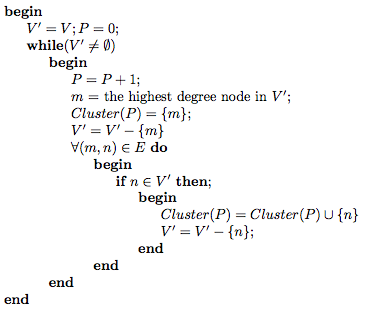
\includegraphics[height=25em]{distk_init}
	\caption{Pseudo-Code for the Distance-k Initialization Algorithm}
\end{center}
\end{figure}

\newpage
\section{Code}
\label{appendix:code}
The Git repository for this project can be found at:
\newline\newline
https://github.com/AriellaRomanov/Clustering

\newpage
\begin{thebibliography}{9}

\bibitem{kernel}
I. Dhillon, Y. Guan, and B. Kulis, ``A Fast Kernel-based Multilevel Algorithm for Graph Clustering,'' \textit{KDD}. Chicago, Ill.: 2005.
 
\bibitem{distK} 
J. Edachery, A. Sen, and F. Brandenburg, ``Graph Clustering Using Distance-k Cliques,'' Arizona State University, 1999.
 
\bibitem{kmeans} 
K. Nazeer and M. Sebastian, ``Improving the Accuracy and Efficiency of the k-means Clustering Algorithm,'' 
\textit{Proceedings of the World Congress on Engineering}. London, U.K.: 2009.

\end{thebibliography}

\begin{comment}
\begin{figure}[!htb]
\begin{center}
	\includegraphics[height=20em]{puppy.png}
	\caption{T-Test for Relative Fitness with Parsimony Pressures 0.2 and 0.3}
	\label{tTestMLR}
\end{center}
\end{figure}
\end{comment}

\end{document}